\documentclass{beamer}
\usepackage[utf8]{inputenc}
\usepackage[T1]{fontenc}
\usepackage{hyperref}
\usepackage[french]{babel}

\hypersetup{pdfpagemode=FullScreen}
\usetheme{Warsaw}
\title{Vino \& plaisir}
\author{Alexandre \and Charef \and Fatemeh \and José }
\setbeamertemplate{section in toc}[ball unnumbered]

\begin{document}
 
\frame{\titlepage}

\begin{frame}{Table des matières}
\tableofcontents
\end{frame}


\section{Structure du MVC}
\begin{frame}
\frametitle{Structure du MVC}
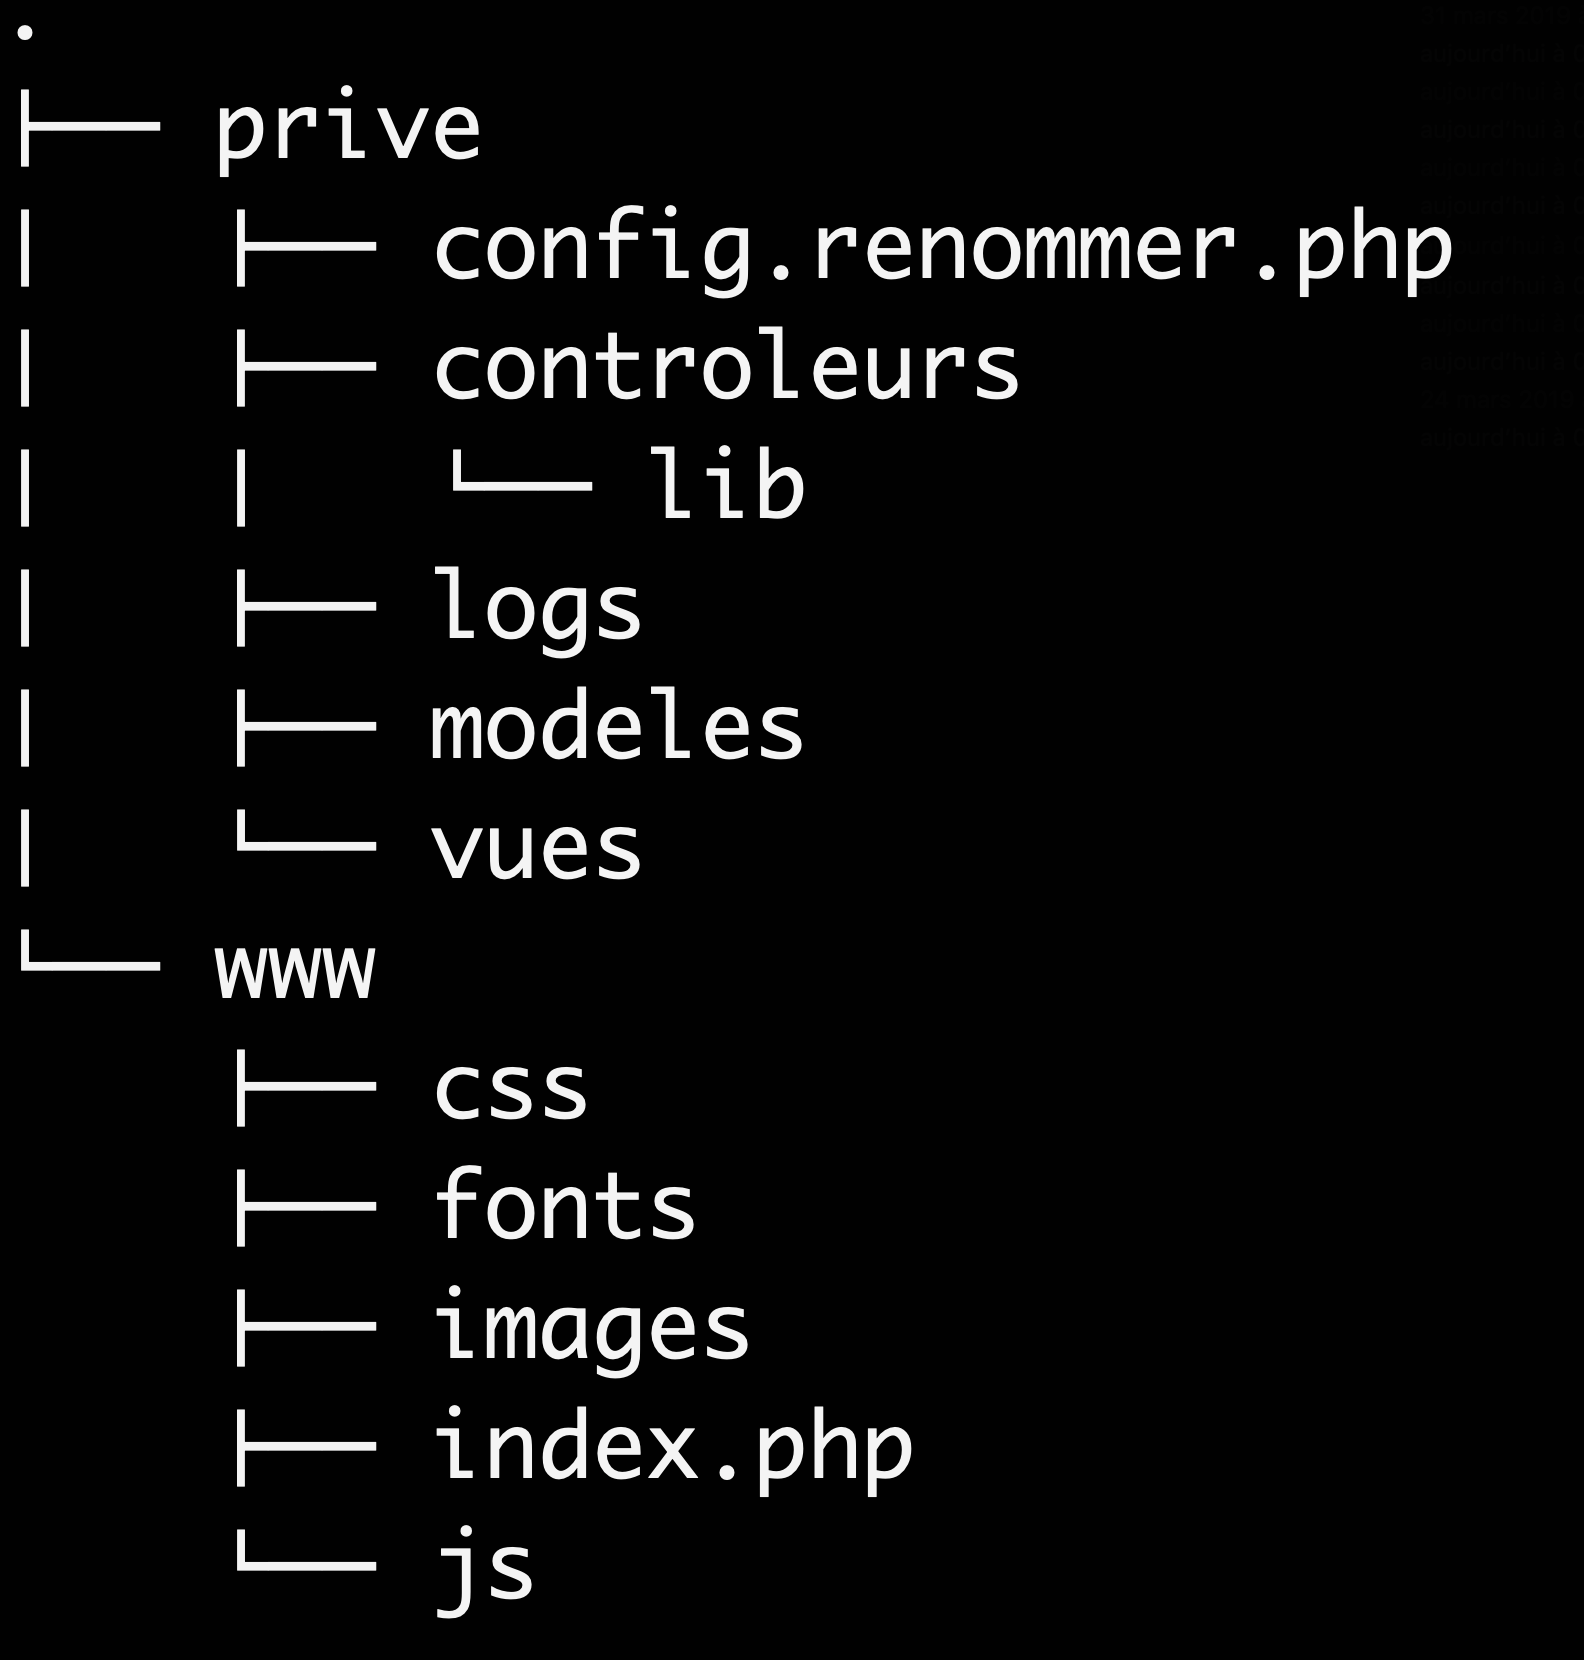
\includegraphics[width=.8\textheight]{tree}
\end{frame}


\section{User stories}
\begin{frame}
\frametitle{User stories}
\begin{enumerate}
	\item En tant qu’administrateur, je peux importer les bouteilles du site de la SAQ;
	\item En tant qu’usager, je peux me créer un compte et le gérer;
	\item En tant qu’usager, je peux créer plusieurs celliers;
	\item En tant qu’usager, je peux gérer mon cellier personnel (ajout, modification, retrait de bouteille);
\end{enumerate}
\end{frame}

\begin{frame}
\begin{enumerate}
	\setcounter{enumi}{4}
	\item En tant qu’usager, je peux ajouter des bouteilles \og non listées \fg{} dans mon cellier;
	\item En tant qu’usager, je peux laisser des notes de dégustation sur les bouteilles que j’ai consommées.
	\item En tant qu’usager, je peux faire des recherches dans mon cellier;
	\item En tant qu’usager, je peux partager sur les réseaux sociaux les bouteilles que j’ai achetées ou bues.
	\item En tant qu’usager, je peux créer une liste d’achat.
\end{enumerate}
\end{frame}

\section{L’application web}
\begin{frame}
\frametitle{L’application web}
\href{http://vino.webportfolio.ca/}{vino.webportfolio.ca}
\end{frame}

\end{document}

